\documentclass{article}

\usepackage{amsmath, amssymb}
\usepackage{float}
\usepackage{graphicx}
\usepackage{subcaption}
\usepackage{color}

\usepackage{listings}


\definecolor{dkgreen}{rgb}{0,0.6,0}
\definecolor{gray}{rgb}{0.5,0.5,0.5}
\definecolor{mauve}{rgb}{0.58,0,0.82}

\lstset{frame=tb,
  language=python,
  aboveskip=3mm,
  belowskip=3mm,
  showstringspaces=false,
  columns=flexible,
  basicstyle={\small\ttfamily},
  numberstyle=\color{gray},
  keywordstyle=\color{blue},
  commentstyle=\color{dkgreen},
  stringstyle=\color{mauve},
  breaklines=true,
  breakatwhitespace=true,
  tabsize=3,
}
%

\addtolength{\topmargin}{-.875in}
\addtolength{\textheight}{1.75in}


\title{Project report - week 4, 5}

\begin{document}
	\maketitle
	\section{Introduction}
		\subsection{Autoencoder}
			An autoencoder is a neural network trained to encode and then decode data.
			In this case the autoencoder was meant to handle image data.
			The network consist of two parts, the encoder, responsible - as the name says - for encoding the data, and decoder recovering original image.
			Encoder was built using three dense layers with decreasing neuron count - 1024, 128, 2.
			Decoder was reversed with dense layers of increasing sizes - 128, 1024, 49152(original size).
			Network was trained using original images as target.
		\subsection{Encoder}
			After training, the encoder part of network was used to encode images into 2 values.
			While reduction accounted for large data loss, it allowed for comparison between all of the images relatively quickly by measuring their geometric distance.
	\section{Results}
		\begin{figure}[h!]
			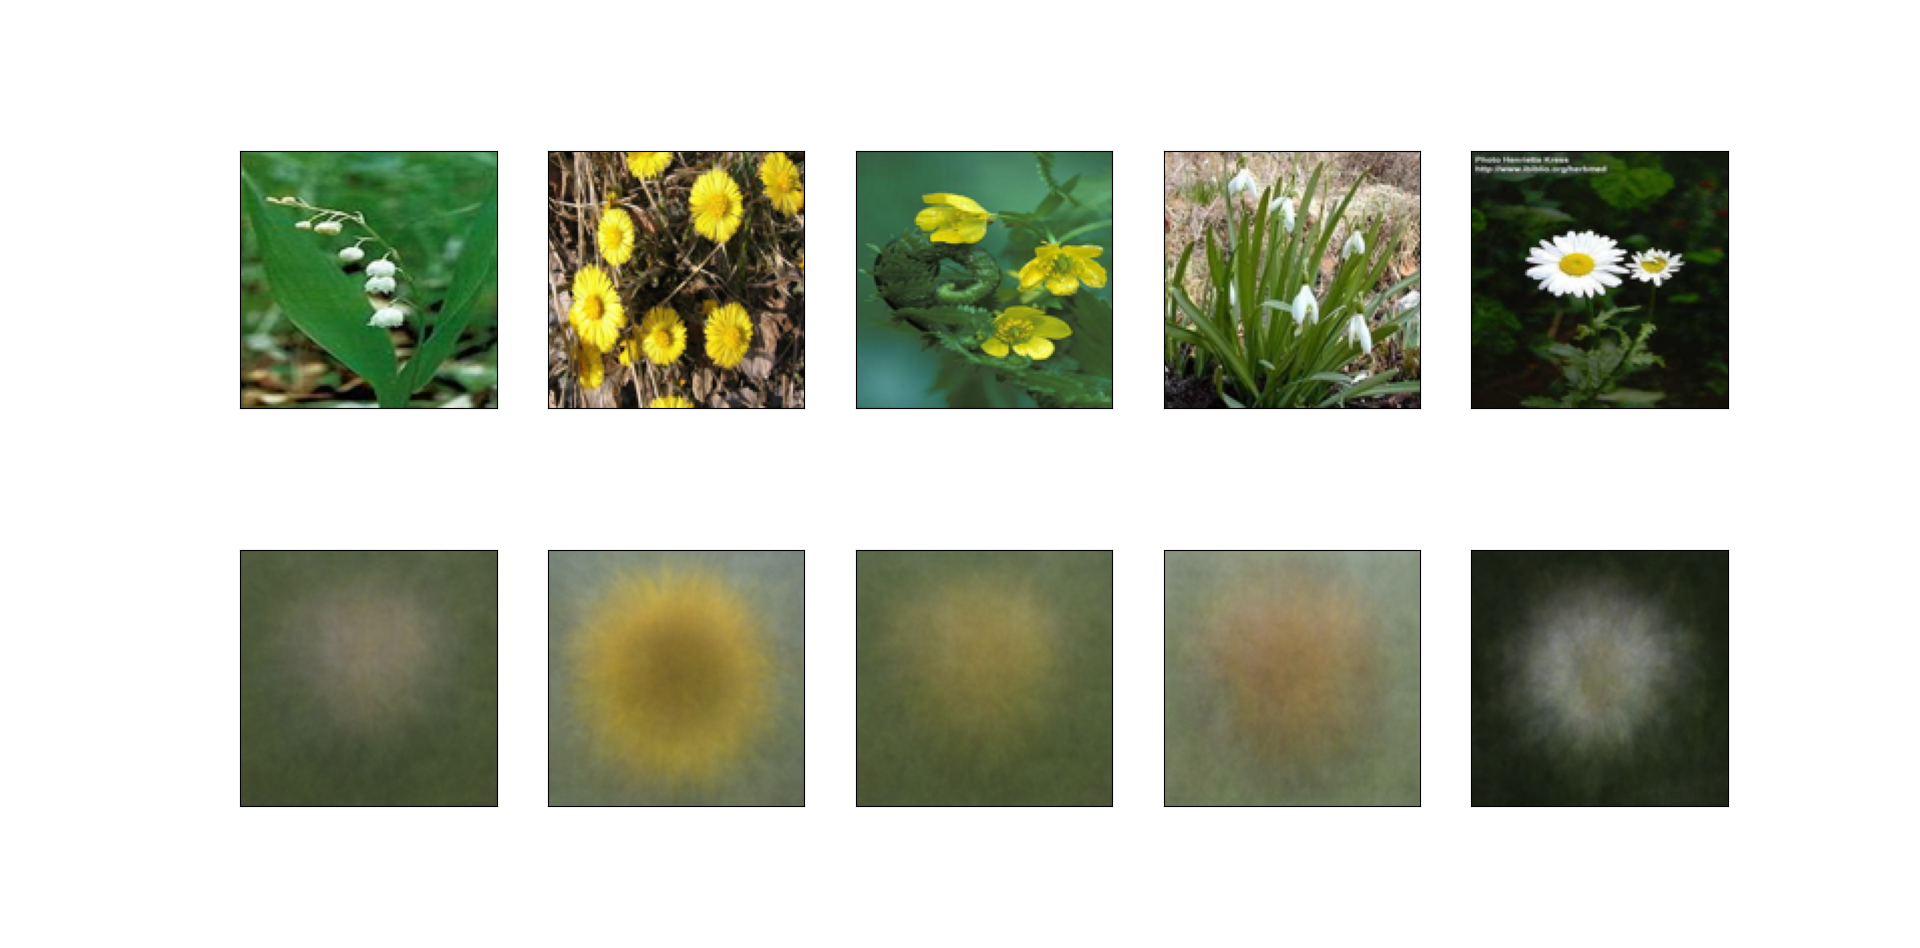
\includegraphics[width = \textwidth]{img/Figure_1}
			\caption{Randomly selected images before and after autoencoding. The only remaining information is color and basic shape (in better cases).}
		\end{figure}
		\pagebreak
		\begin{figure}[t!]
			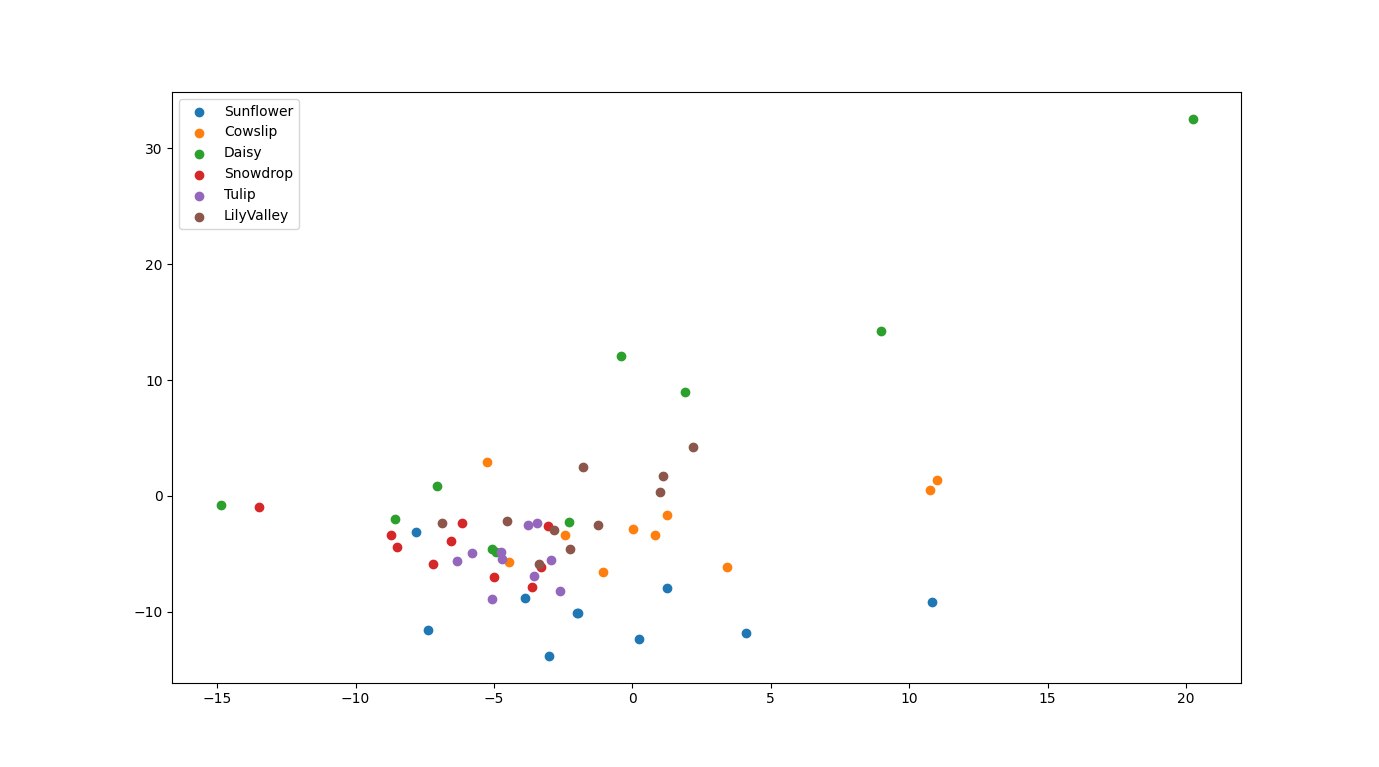
\includegraphics[width = \textwidth]{img/Figure_2}
			\caption{Results of plotting encoded images in two dimensions. While overlapping, it's possible to distinguish different groups. Only few samples of selected flowers were included for readability.}
		\end{figure}  \mbox{}
\end{document}